\documentclass[11pt]{article}

\usepackage{acl2014}
\usepackage{times}
\usepackage{url}
\usepackage{latexsym}
\usepackage{amsmath}
\usepackage{amssymb}
\usepackage{graphicx}
\usepackage{multicol}

\newcommand{\Eq}[1]{Equation (\ref{eq:#1})}
\newcommand{\eq}[1]{Equation (\ref{eq:#1})}
\newcommand{\eqlabel}[1]{\label{eq:#1}}
\newcommand{\Fig}[1]{Figure~\ref{fig:#1}}
\newcommand{\fig}[1]{Figure~\ref{fig:#1}}
\newcommand{\figlabel}[1]{\label{fig:#1}}

\newcommand{\etal}{\emph{et al.}}

\DeclareMathOperator*{\argmax}{arg\,max}
\DeclareMathOperator*{\argmin}{arg\,min}

\title{Collaborative Topic Modeling for Scientific Article Recommendations}

\author{Daniel Foreman-Mackey \\ {\tt danfm@nyu.edu} \\}

\begin{document}
\maketitle

\begin{abstract}
The code is available on GitHub at \url{https://github.com/dfm/clda} under the
terms of the MIT License.
\end{abstract}

\section{Introduction}

\section{Implicit feedback collaborative filtering}

In this problem, we don't have explicit feedback (such as starred ratings)
from the users.
Instead, we have only implicit feedback: is the article in the bibliography or
not?
To approach this problem, I implemented the algorithm described by Hu, Koren
\& Volinsky~\shortcite{icf}.
The main idea behind this algorithm is that they treat the null entries in the
``ratings'' matrix as low-confidence negative ratings and the observed entries
as higher-confidence positive indicators.
Then, they perform the full probabilistic matrix factorization on this system.
Specifically, the log-likelihood function is
\begin{eqnarray}
\mathcal{L} &=& -\sum_{i,j}
                c_{ij}\,(r_{ij}-\mathbf{u}_i^\mathrm{T}\,\mathbf{v}_j)^2
\nonumber\\
&& - \lambda_u\,\sum_i \mathbf{u}_i^\mathrm{T}\,\mathbf{u}_i
 - \lambda_v\,\sum_j \mathbf{v}_j^\mathrm{T}\,\mathbf{v}_j
\end{eqnarray}
where $\mathbf{u}_i$ is the latent representation of user $i$,
$\mathbf{v}_j$ is the latent representation of the document $j$, and $c_{ij}$
is the model confidence in the rating $r_{ij}$.
In this particular context, our model will have $r_{ij} = 1$ if document $j$
is in user $i$'s library and $r_{ij} = 0$ otherwise.

If we define the matrices of user and document representations $U$ and $V$,
then the maximum likelihood result of this system is
\begin{eqnarray}
\mathbf{u}_i &\gets& (V\,C_i\,V^\mathrm{T}+\lambda_u)^{-1}\,
                     V\,C_i\,\mathbf{r}_i
\quad \mathrm{and} \nonumber \\
\mathbf{v}_j &\gets& (U\,C_j\,U^\mathrm{T} + \lambda_v)^{-1}\,U\,C_j\,
                     \mathbf{r}_j
\end{eqnarray}
where $C_{i/j}$ is the diagonal matrix of confidences and $\mathbf{r}_{i/j}$
is the vector of ratings for user $i$/document $j$.

I also chose to use the same confidence model as Hu \etal~(2008)
\begin{eqnarray}
c_{ij} &=& 1+\alpha\,r_{ij}
\end{eqnarray}
where $\alpha$ is a free parameter.

\section{Latent Dirichlet allocation}

\section{Collaborative LDA}

In this model, the maximum likelihood updates are \cite{ctr}
\begin{eqnarray}
\mathbf{u}_i &\gets& (V\,C_i\,V^\mathrm{T}+\lambda_u)^{-1}\,
                     V\,C_i\,\mathbf{r}_i
\quad \mathrm{and} \\
\mathbf{v}_j &\gets& (U\,C_j\,U^\mathrm{T} + \lambda_v)^{-1}\,(U\,C_j\,
                     \mathbf{r}_j + \lambda_v\,\theta_j) \nonumber
\end{eqnarray}

\section{Experiments}

\begin{figure}
\centering
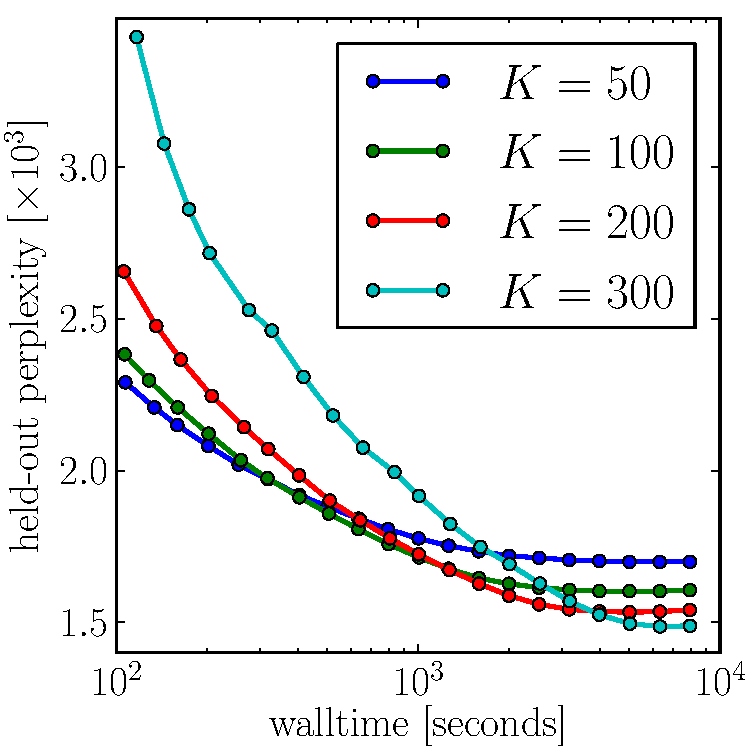
\includegraphics[width=0.4\textwidth]{lda-results-k.pdf}
\caption{%
The held-out perplexity as a function of runtime for different model
topic model complexities.
\figlabel{lda-results}}
\end{figure}

\begin{figure}
\centering
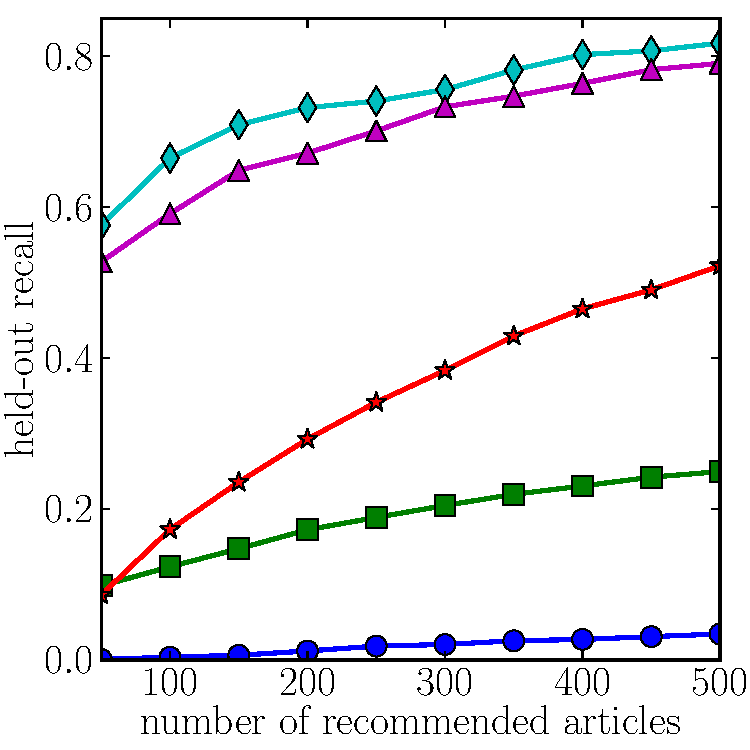
\includegraphics[width=0.4\textwidth]{results.pdf}
\caption{%
The recall curves for the set of tested models.
From worst to best, the models are: random (blue dots), tf--idf (green
squares), LDA (red stars), CLDA (purple triangles), and ICF (cyan diamonds).
See the text for descriptions of these models.
\figlabel{results}}
\end{figure}

\newpage
\begin{multicols}{2}
\begin{figure*}
\centering
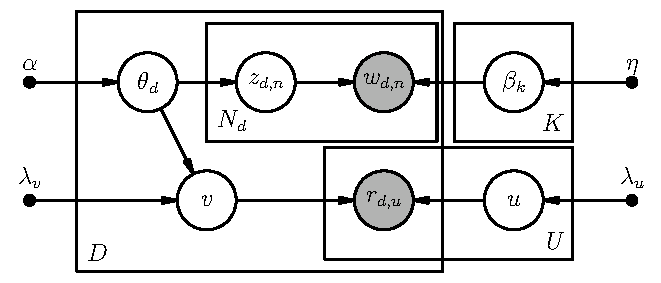
\includegraphics{clda.pdf}
\caption{%
CLDA
\figlabel{clda}}
\end{figure*}
\end{multicols}

\newpage
\section{Honor Pledge}
I pledge my honor that all the work described in this report is solely mine
and that I have given credit to all third party resources that I have used.

\begin{thebibliography}{}

\bibitem[\protect\citename{Hoffman, Blei \& Bach}2010]{ovlda}
M. Hoffman, D. Blei, \& F. Bach.
\newblock{{\bf Online learning for latent Dirichlet allocation}}
\newblock{\emph{Neural Information Processing Systems},}
\newblock{2010.}

\bibitem[\protect\citename{Hu, Koren \& Volinsky}2008]{icf}
Y. Hu, Y. Koren, \& C. Volinsky.
\newblock{{\bf  Collaborative filtering for implicit feedback datasets}}
\newblock{\emph{Proceedings of the 2008 Eighth IEEE International Conference
                on Data Mining},}
\newblock{2008.}

\bibitem[\protect\citename{Wang \& Blei}2011]{ctr}
C. Wang \& D. Blei.
\newblock{{\bf Collaborative topic modeling for recommending scientific
           articles}}
\newblock{\emph{Knowledge Discovery and Data Mining},}
\newblock{2011.}

\end{thebibliography}

\end{document}
